\documentclass{article}
\usepackage[utf8]{inputenc}
\usepackage{amsmath}
\usepackage{xcolor}
\usepackage[top=2cm, bottom=2cm, left=2cm, right=2cm]{geometry}
\setlength\parindent{0pt}

\usepackage{listings}
%\usepackage{color}
\usepackage{graphicx}
\usepackage{float}
\usepackage{caption}

\usepackage{verbatim}
\let\oldv\verbatim
\let\oldendv\endverbatim

%\userpackage{minted}

\definecolor{dkgreen}{rgb}{0,0.6,0}
\definecolor{gray}{rgb}{0.5,0.5,0.5}
\definecolor{mauve}{rgb}{0.58,0,0.82}
\definecolor{light-gray}{gray}{0.95}


\lstset{frame=tb,
  language=Java,
  aboveskip=6mm,
  belowskip=6mm,
  showstringspaces=false,
  columns=flexible,
  basicstyle={\small\ttfamily},
  numbers=none,
  numberstyle=\tiny\color{gray},
  keywordstyle=\color{blue},
  commentstyle=\color{dkgreen},
  stringstyle=\color{mauve},
  breaklines=true,
  breakatwhitespace=true,
  tabsize=3,
  backgroundcolor=\color{light-gray},
  language=Matlab
}

%\usepackage{natbib} replaced by line below to make refernces work
\usepackage[square,sort,comma,numbers]{natbib}
\usepackage[nottoc,numbib]{tocbibind} %to get references in table of contants
\usepackage{graphicx}

\usepackage{bm}

\usepackage{hyperref}
\hypersetup{
	colorlinks,
	citecolor=black,
	filecolor=black,
	linkcolor=black,
	urlcolor=black
}

\usepackage{mdframed}
\usepackage{lipsum} % for creating dummy text
\mdfdefinestyle{MyFrame}{%
	linecolor=black,	
	backgroundcolor=gray!20!white,
	skipbelow = 8mm,
	skipabove = 8mm}

\usepackage{scrextend}

\title{Fys4150\\Project 3\\ }
\author{Peter Killingstad and Karl Jacobsen\\
\\
\url{https://github.com/kaaja/fys4150}}
\begin{document}
	
\maketitle

\section*{Note to instructurs about Github repository}
If the above Github-link does not work, it is eighter because you have not yet accepted our invite to the repository, or you have not yet provided us with an e-mail adress available at Github so that we can invite you. If the latter applies to you, please send us an e-mail with an e-mailadress available in Github or your Github username so that we can send you an invite. Our e-mailadresses: peter.killingstad@hotmail.com, karljaco@gmail.com.

\section*{Abstract}


\section{Introduction}


\section{Theory}



\section{Results}

\subsection{Sun-Earth Forward Euler}

\begin{minipage}{.49\textwidth} 
	\begin{figure}[H]
		\centering
		\includegraphics[width=0.99\textwidth]{/home/karl/doc/subj/att/fys4150/project3/resultsKeep/plots/sunEarthTimes.png}
		\caption{Sun-Earth system. Effect of $\Delta t$ over a 10 year period. \\ \textit{The Forward Euler method seems to converge for the two smallest $\Delta t$}}
		\label{1}
	\end{figure}
\end{minipage}\hfill
\begin{minipage}{.49\textwidth} 
	\begin{figure}[H]
		\centering
		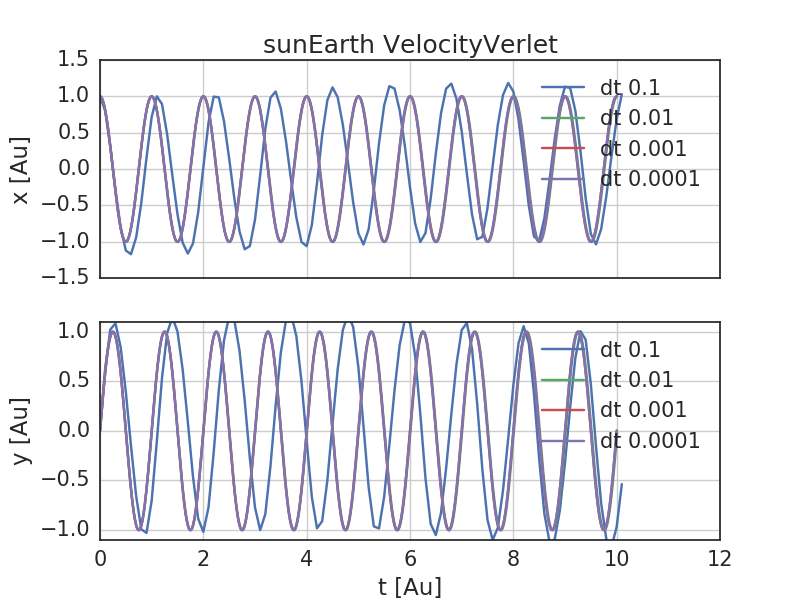
\includegraphics[width=0.99\textwidth]{/home/karl/doc/subj/att/fys4150/project3/resultsKeep/plots/sunEarthTimesVelocityVerlet.png}
		\caption{Sun-Earth system. Effect of $\Delta t$ over a 10 year period. \\ \textit{The Velocity verlet method seems to converge faster than Forward Euler}}
		\label{1}
	\end{figure}
\end{minipage}\hfill
\vspace{2ex}


\begin{minipage}{.49\textwidth} 
	\begin{figure}[H]
		\centering
		\includegraphics[width=0.99\textwidth]{/home/karl/doc/subj/att/fys4150/project3/resultsKeep/plots/sunEarthfinalTime10N1000.png}
		\caption{Sun-Earth system. Forward Euler. 10 years \\ \textit{Non-circulat orbits when time step is large.}}
		\label{1}
	\end{figure}
\end{minipage}\hfill
\begin{minipage}{.49\textwidth} 
	\begin{figure}[H]
		\centering
		\includegraphics[width=0.99\textwidth]{/home/karl/doc/subj/att/fys4150/project3/resultsKeep/plots/sunEarthfinalTime10000N10000000.png}
		\caption{Sun-Earth system. Forward Euler. 10 000 years. \\ \textit{For $\Delta t = 0.01$, the forward Euler seems to give circular orbits, but we can see that the solution changes.}}
		\label{1}
	\end{figure}
\end{minipage}\hfill
\vspace{2ex}

\begin{minipage}{.49\textwidth} 
	\begin{figure}[H]
		\centering
		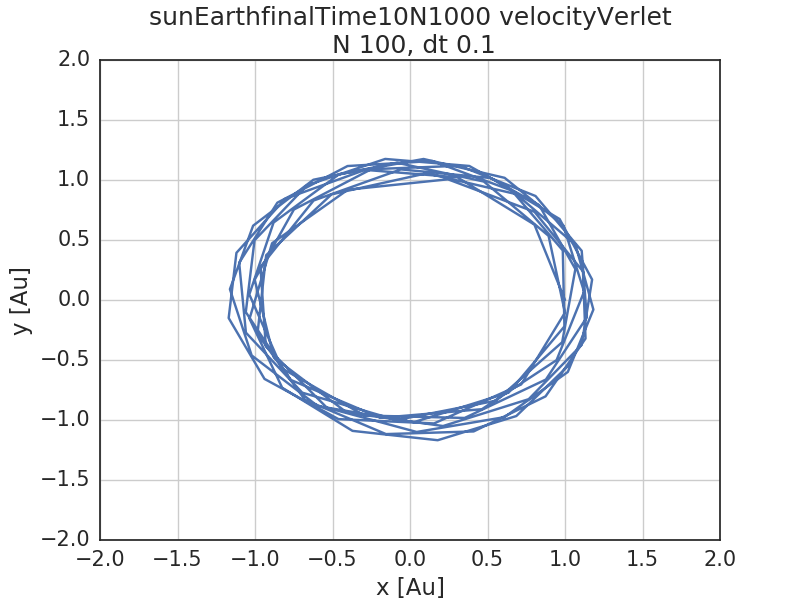
\includegraphics[width=0.99\textwidth]{/home/karl/doc/subj/att/fys4150/project3/resultsKeep/plots/sunEarthfinalTime10N1000VelocityVerlet.png}
		\caption{Sun-Earth system. Velocity Verlet. 10 years. \\ \textit{Large time step gives bad solutions also for Velocity Verlet.}}
		\label{1}
	\end{figure}
\end{minipage}\hfill
\begin{minipage}{.49\textwidth} 
	\begin{figure}[H]
		\centering
		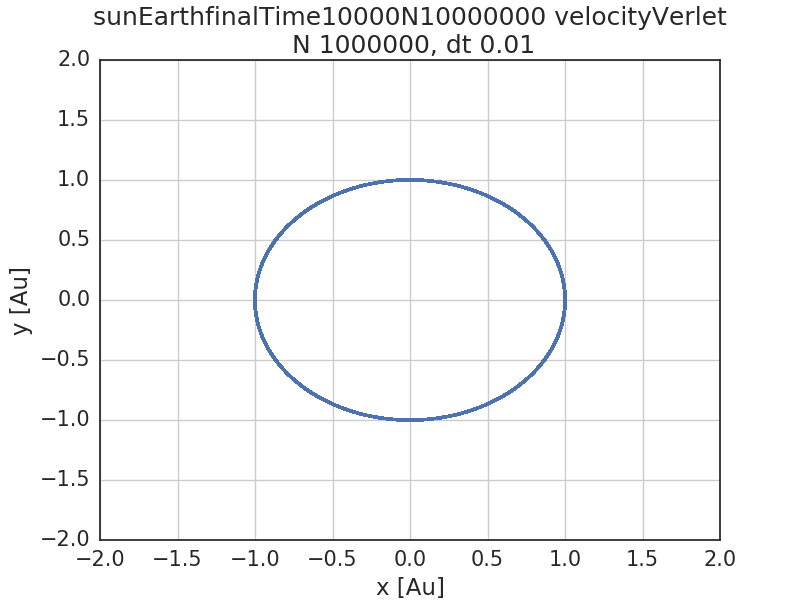
\includegraphics[width=0.99\textwidth]{/home/karl/doc/subj/att/fys4150/project3/resultsKeep/plots/sunEarthfinalTime10000N10000000VelocityVerlet.png}
		\caption{Sun-Earth system. Velocity Verlet. 10 000 years. \\ \textit{For velocity Verlet, the orbits seems to stay more circular compared to Forward Euler.}}
		\label{1}
	\end{figure}
\end{minipage}\hfill
\vspace{2ex}

\begin{minipage}{.49\textwidth} 
	\begin{figure}[H]
		\centering
		\includegraphics[width=0.99\textwidth]{/home/karl/doc/subj/att/fys4150/project3/resultsKeep/plots/sunEarthEnergy.png}
		\caption{Sun-Earth system. Total Energy divided by total energy first time step. Forward Euler. 10 years. \\ \textit{Energy is not preserved with the Forward Euler method}}
		\label{1}
	\end{figure}
\end{minipage}\hfill
\begin{minipage}{.49\textwidth} 
	\begin{figure}[H]
		\centering
		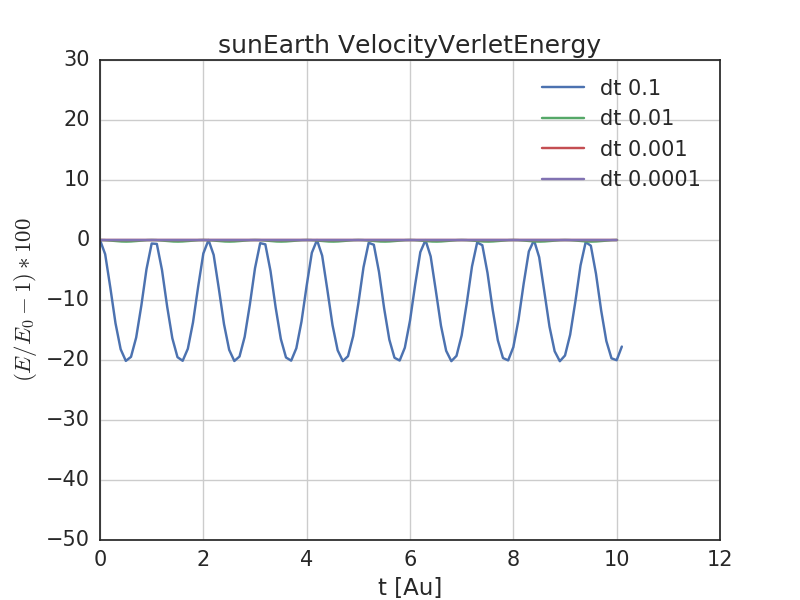
\includegraphics[width=0.99\textwidth]{/home/karl/doc/subj/att/fys4150/project3/resultsKeep/plots/sunEarthEnergyVelocityVerlet.png}
		\caption{Sun-Earth system. Total Energy divided by total energy first time step. Velocity Verlet. 10 years. \\ \textit{Energy is preserved in Velocity Verlet provided fine enough time step. }}
		\label{1}
	\end{figure}
\end{minipage}\hfill
\vspace{2ex}


\begin{minipage}{.49\textwidth} 
	\begin{figure}[H]
		\centering
		\includegraphics[width=0.99\textwidth]{/home/karl/doc/subj/att/fys4150/project3/resultsKeep/plots/sunEarthAngularMomentum.png}
		\caption{Sun-Earth system. Angular momentum divided by angular momentum first time step. Forward Euler. 10 years. \\ \textit{Angular momentum seems to be conserverd for the finest time step.}}
		\label{1}
	\end{figure}
\end{minipage}\hfill
\begin{minipage}{.49\textwidth} 
	\begin{figure}[H]
		\centering
		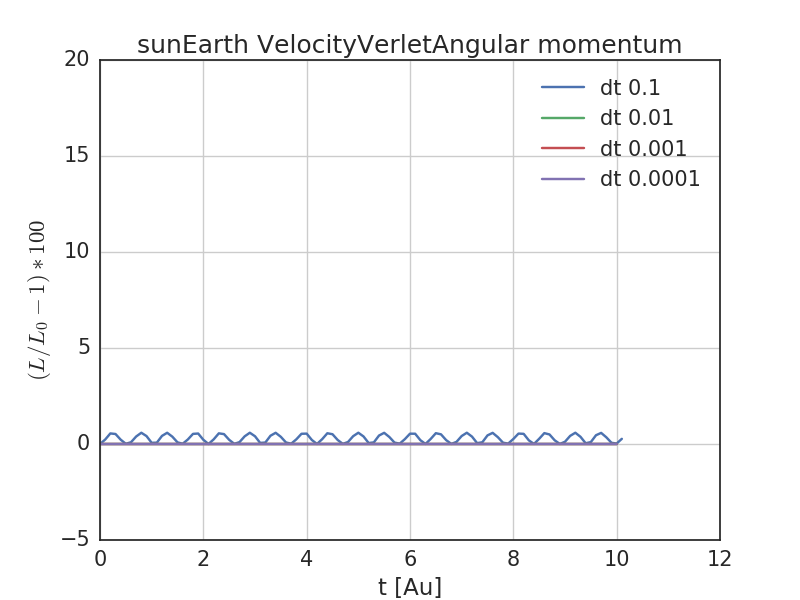
\includegraphics[width=0.99\textwidth]{/home/karl/doc/subj/att/fys4150/project3/resultsKeep/plots/sunEarthAngularMomentumVelocityVerlet.png}
		\caption{Sun-Earth system. Angular momentum divided by angular momentum first time step. Velocity Verlet. 10 years. \\ \textit{Angular momentum is conserverd given suffiently fine time steps. Conservation achieved faster than with Forward Euler.}}
		\label{1}
	\end{figure}
\end{minipage}\hfill
\vspace{2ex}

\begin{minipage}{.49\textwidth} 
	\begin{figure}[H]
		\centering
		\includegraphics[width=0.99\textwidth]{/home/karl/doc/subj/att/fys4150/project3/resultsKeep/plots/sunEarthsupNorm.png}
		\caption{Sun-Earth system. Sup-norm total energy. Forward Euler. \\ \textit{Forward Euler's sup-norm goes like $\mathcal{O}(\Delta t)$}}
		\label{1}
	\end{figure}
\end{minipage}\hfill
\begin{minipage}{.49\textwidth} 
	\begin{figure}[H]
		\centering
		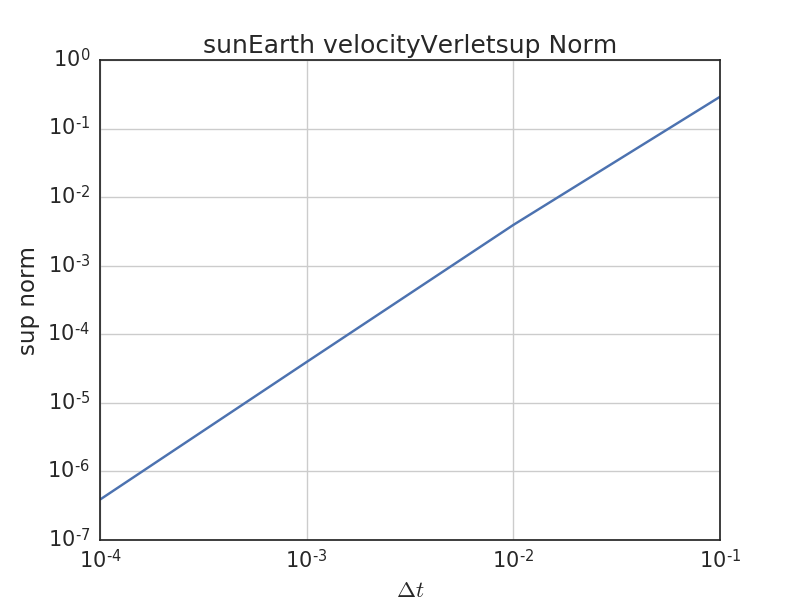
\includegraphics[width=0.99\textwidth]{/home/karl/doc/subj/att/fys4150/project3/resultsKeep/plots/sunEarthsupNormVelocityVerlet.png}
		\caption{Sun-Earth system. Sup-norm total energy. Velocity Verlet \\ \textit{The sup-norm in energy for Velocity Verlet goes one higher order than Forward Euler}}
		\label{1}
	\end{figure}
\end{minipage}\hfill
\vspace{2ex}

\begin{minipage}{.49\textwidth} 
	\begin{figure}[H]
		\centering
		\includegraphics[width=0.99\textwidth]{/home/karl/doc/subj/att/fys4150/project3/resultsKeep/plots/sunEarthsupNormAngularMomentum.png}
		\caption{Sun-Earth system. Sup-norm Angular Momentum. Forward Euler \\ \textit{Forward Euler's sup-norm for angular momentum goes like $\mathcal{O}(\Delta t^2)$}.}
		\label{1}
	\end{figure}
\end{minipage}\hfill
\begin{minipage}{.49\textwidth} 
	\begin{figure}[H]
		\centering
		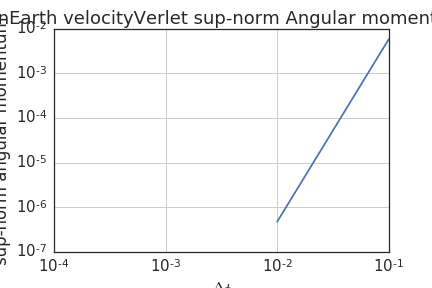
\includegraphics[width=0.99\textwidth]{/home/karl/doc/subj/att/fys4150/project3/resultsKeep/plots/sunEarthsupNormAngularMomentumVelocityVerlet.png}
		\caption{Sun-Earth system. Sup-norm Angular momentum. Velocity Verlet \\ \textit{Velocity Verlet's sup-norm error less than $10^{-12}$ like $\mathcal{O}(\Delta t^4)$.}}
		\label{1}
	\end{figure}
\end{minipage}\hfill
\vspace{2ex}

\section{Conclusions}






\section{Feedback}
\subsection{Project 1}
This project has been extremely educational. We learned about about c++, especially pointers and dynamic memory allocoation. Also which for us was a well forgotten subject, we learned about dangerous of numerical round-off errors. \\

We feel the size of the project is large, much larger than typical assignments in other courses. However, the quality and quantity of the teaching without a doubt made the workload managable. The detailed lectures, combined with the fast and good respones on Piazza helped a lot!\\

We think the project could have gone even smoother, if we on the 2nd lab-session had learned basic branching in Github. We used a considerable amount of time finding out of this.\\

All in all, two thumbs up!

\subsection{Project 2}
\begin{itemize}
	\item  catch: We ended up using a lot of time making this work properly. Still we have some problems with catch and Qt. We think we might had benefited from a demonstration at the lab.
	
	\item We were not able to understand the revised Sturm-Bisection algorithm from Barth et al.'s \cite{barth} paper on the revised Sturm-Bisection. 
	
	\item Apart from the small details above, we are very happy about this project. How would have thought linear algebra could be fun?!
\end{itemize}



\pagebreak
\begin{thebibliography}{9}
	\bibitem{barth} 
	Barth, Martin, Wilkinson (1967)
	Calculation of eigenvalues of a symmetric tridiagonal matrix by the method of bisection. \textit{Numeriche mathematik 9, 386 - 393 (1967)}
	
	\bibitem{MHJ} 
	Hjorth-Jensen, M.(2015)
	Computational physics. Lectures fall 2015. 
	\url{https://github.com/CompPhysics/ComputationalPhysics/tree/master/doc/Lectures}
	
	\bibitem{MHJProject2} 
	Hjorth-Jensen, M.(2017)
	Project 2, fys4150 2017.
	\url{https://github.com/CompPhysics/ComputationalPhysics/blob/master/doc/Projects/2017/Project2/pdf/Project2.pdf}
	
	\bibitem{kiusalaas} 
	Kiusalaas, J.(2013)
	Numerical Methods in Engineering with Python 3. 3rd edition.
	
	\bibitem{taut} 
	Taut, M. (1993)
	Two electrons in an external oscillator potential: Particular analytic solutions of a Coulomb correlation problem \textit{Phys. Rev. A 48, 3561 (1993).}
	
	


\end{thebibliography}


\end{document}
